% Does `(\tag v1)` name the node `av1`?
%
% A foreach body writes `\node (\tag v1) at ... {}` with \tag = a, and the author's later
% `\draw (av1)` has no space. TeX swallows the blank that delimits a control word, so the two are the
% same node. If that is right this page compiles with no `Reference ... undefined` in the log; if the
% space survived as part of the name, `(av1)` is an unknown coordinate and the warning appears.
\documentclass{article}
\usepackage{tikz}
\begin{document}
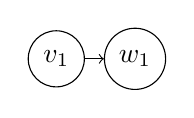
\begin{tikzpicture}
  \def\tag{a}
  \node[circle,draw] (\tag v1) at (0,0) {$v_1$};
  \node[circle,draw] (\tag w1) at (1,0) {$w_1$};
  \draw[->] (av1) -- (aw1);
\end{tikzpicture}
\end{document}
